\documentclass[../report.tex]{subfiles}

\begin{document}
\graphicspath{{img/}{../img/}}

\section{SCRUM men... Ikke helt}


\paragraph{Hvad er SCRUM?}
SCRUM er en agil software udviklings metode, hvis hovedm�l er at kunne h�ndtere �ndringer i kravspecifikationen mens udviklingen er i gang. Indenfor godtagelse af krav�ndringer er SCRUM mods�tningen til vandfaldsmodellen, som ikke tager sig p�nt i et milj� med mange krav �ndringer.

\paragraph{SCRUM men... Hvad mangler s�?} I vores target projekt bruger vi SCRUM ? men ikke SCRUM i dets fulde forstand. I det projekt har vi valgt at k�re l�st p� nogle af SCRUMS discipliner, fordi vi var enige om at de ikke gav meget mening for en projekt gruppe der kun m�des et par gange om ugen.\\


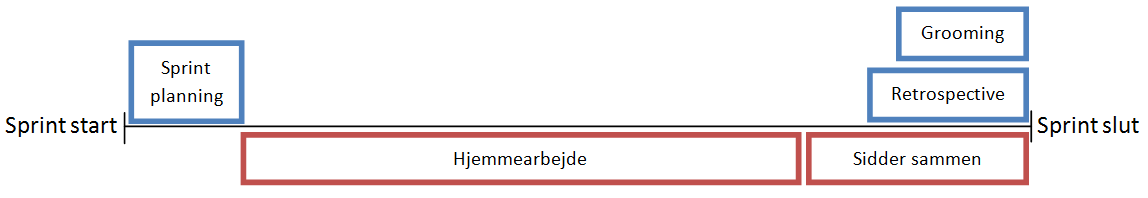
\includegraphics[scale=0.8]{SCRUMtimeLine.png}\\

\begin{tabular}{c|p{10cm}}
\textbf{Aktiviteter}  & \textbf{�ndringer} \\
SCRUM roller & I et eksamensprojekt er det urealistisk at have en person til kun at v�re product owner. I vores target projekt er product owner ene og alene ansvarlig for kommunikation med stakeholders og prioritering af product items, men han er ogs� udvikler i SCRUM teamet     \\ 
 & \\
SCRUM Board & SCRUM boardet er den centrale oversigt over hvad der skal laves og er lavet. Boardet fungere efter vores erfaringer ogs� som stor motivations-faktor. Da vi i vores target projekt ikke har et fast lokale, er et fysisk board dog ikke muligt, og vi bruger i stedet online v�rkt�jet Trello\footnote{Trello.com} \\
 & \\
Standup meeting & Da vi i vores target projekt arbejder ofte selvst�ndigt \\
 & \\
 & \\
 & \\
\end{tabular} 


\end{document}